\section{Previous Work}

\subsection{Global Change Master Directory}
The Global Change Master Directory (GCMD) is a metadata repository used by the National Aeronautics and Space Administration (NASA) to store records of its available data sets \cite{Miled:2001:GCM:372202.372324}.
GCMD employs a taxonomy of keywords to make NASA Earth Science data sets searchable.
These words tag and label datasets into strictly defined categories \cite{GCMDKey}.
The management team stored early versions of the keywords in Excel spreadsheets, later using a centralized distribution system, but data is not available prior to June 12, 2012.
The Key Management Service (KMS) now serves the keywords directly in a variety of formats.
Other than the initial version, named `June122012', versions are given a dot-decimal identifier.
According to the \textit{Keyword Governance and Community Guide Document}, ``Full GCMD keywords list releases get a new major version number (e.g., 8.0). Incremental releases for updates to topics, terms, and variables get a new minor version number (e.g., 8.1),” \cite{gcmd_gov}.

Each keyword corresponds to a Universally Unique Identifier (UUID), and when combined with a web namespace, resolves to a data description of the keyword.
Every identifier can be referred to per version by including the version's number at the web identifier's end, meaning that identifiers are consistent across versions.
The namespace, UUID, and version form a versioned keyword's Uniform Resource Identifier.
The taxonomy uses the concepts \textit{skos:Broader} and \textit{skos:Narrower}, where skos refers to the Simple Knowledge Organization System (SKOS) ontology name space, to form a tree hierarchy \cite{skos}.
The tree's root is the keyword, "Science Keywords."
The data set provides an interesting study case due its long sequence of versions and ready use of linked-data technology \cite{Stevens2016}.

\subsection{Dot-Decimal Identifiers}
A dot-decimal identifier is a series of numbers joined together by a decimal point with the left-most number signifying a commonality across major features and the right-most number signifying a commonality across the most minor features, as seen in Figure \ref{dot_decimal}.
\begin{figure}
	\centering
	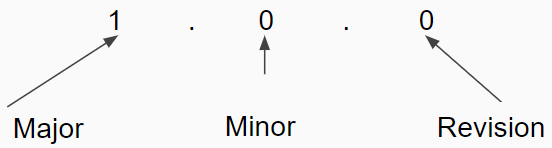
\includegraphics[scale=0.9]{dot_decimal.png}
	\caption{A dot-decimal identifier is broken into a series of number separated by decimals.  The left-most number indicates a grouping over major features.  Intervals moving to the right decrease in significance.  The third interval often has different names, but we have chosen to refer to the interval as the revision number.}
	\label{dot_decimal}
\end{figure}
The amount of change between two versions is determined by finding the left-most interval at which the identifiers differ.
Because the identifiers traditionally denote a version's location in a sequence, only one interval is changed at a time and is only incremented by one.